\chapter{Code Review}
As in assignment one, the model building of the problem has already been conducted in the statement of the task. Since the solution of the problem is also similar to assignment one, big parts of the code are similar.

The biggest changes in are:

\begin{itemize}
\item A time loop to solve the system of linear equations for each time step
\item Inclusion of a surface plot of the Temperature over time and length
\item Plot of a residual
\item Consideration of $\Delta t$ and density in the source terms
\item Consideration of $\Delta t$ and density in the system matrix
\end{itemize}


\section{Time loop}
\lstinputlisting[language=Matlab, firstline=69, lastline=75, caption={Time loop implementation}, label=lst:timeLoop]{code/main.m}

As seen in \autoref{lst:timeLoop}, a further for loop was implemented in which the system of linear equations is solved in line 2. In line 3, the Temperature over the length is written into the j-th row of T\_time, the source terms are recalculated based on the new Temperature in each cell in line 4 and in line 5 the j-th entry of the residual vector is calculated. Line 6 saves the last Temperature for the next calculation of the residual.


%
\section{Surface plot of T}
\lstinputlisting[language=Matlab, firstline=120, lastline=125, caption={Plotting T over x and t}, label=lst:surfPlot]{code/main.m}

\autoref{lst:surfPlot} shows the implementation of a plot of Temperature over time and x. In line 1 a new figure with id 5 is created, then filled with a surface plot in line 2. Line 3, 4  and 5 set labels for the axes and limits on the time axis.

\section{Plotting the residual}
As already seen in \autoref{lst:timeLoop}, a residual vector is filled every time step. This residual is then plotted over time for every mesh size.


\section{Change to the source terms}
Since the source terms are now dependent on the temperature in each cell and the time step, they are updated each time step. The updated code reflects this dependency as seen in \autoref{lst:sourceTerms} line 9. Also sourceTerms now takes the temperature in each cell, the density and the time step as an input.


\lstinputlisting[language=Matlab, firstline=1, lastline=15, caption={Updated sourceTerms function}, label=lst:sourceTerms]{code/sourceTerms.m}

\section{Change to the system matrix}
The system matrix is now dependent on the time step. This is an additional input argument of the function. It is implemented analogous to sourceTerms.




\chapter{Investigation of mesh size}


Mesh size is investigated for a large amount of time steps and a small time step $\Delta t$. This is so that a time-independent solution is reached. The time step chosen was $\Delta t = 0.01 s$, the end time $t_{end} = 10^4 s$. This is equal to $10^6$ iterations. The mesh sizes chosen were 10, 13, 16, 19, 22, and 25 mesh elements. The error over the length at $t = 10^4 s$ can be seen in \autoref{fig:errT}.


\begin{figure}[H]
    \centering
    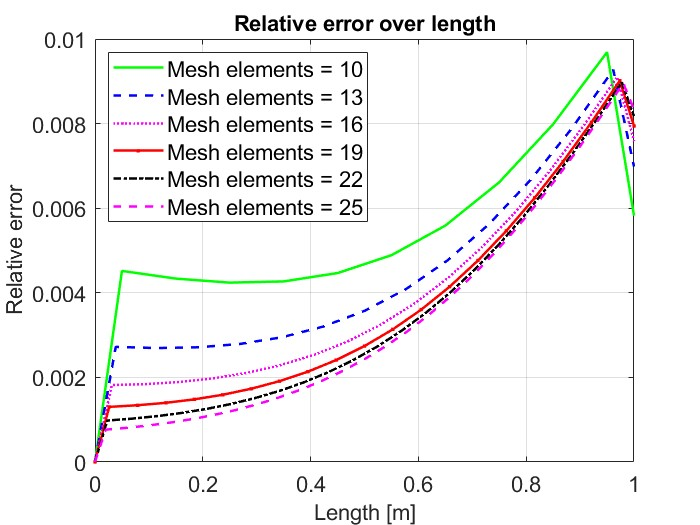
\includegraphics[width=.75\textwidth]{figures/TsmalldtBigtErr.jpg}
    \caption{Relative error to the transient solution over the length of the fin at $t = 10^4 s$}
    \label{fig:errT}
\end{figure}




\begin{figure}[H]
    \centering
    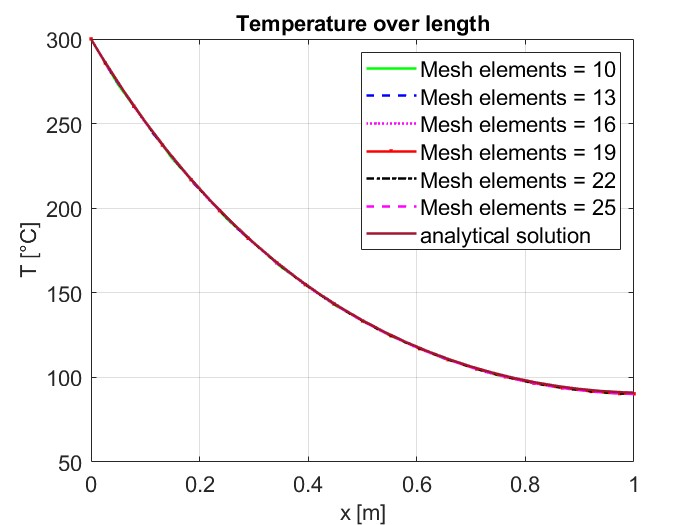
\includegraphics[width=.75\textwidth]{figures/TsmalldtBigt.jpg}
    \caption{Temperature distribution of the transient solution over the length of the fin at $t = 10^4 s$ and the analytical solution}
    \label{fig:T}
\end{figure}

The final temperature distribution as well as the analytical, steady-state solution can be seen in \autoref{fig:T}.

As seen in \autoref{fig:errT} and \ref{fig:T}, the distribution does not depend on mesh size at the chosen time step and end times since the error lies below 1 percent for all meshes, the distributions indistinguishable from the analytical solution. A mesh size of $n = 10$ elements is therefore chosen for further investigations.









